\nextslide{Basics}
\begin{enumerate}
\item{JML, Jack}
\item{Coq}
\item{Purity}
\end{enumerate}

\nextslide{JML and Jack}\small
The {\purple Java Modelling Language} (JML)
is used to annotate the Java programs we want to verify with 
Jack.\\
%Jack use a {\purple weakest precondition calculus} to generate
%the proof obligations.\\
Jack:
\blist
\item An Eclipse plugin
\item Uses a {\purple weakest precondition calculus} to generate proof obligations
\item The proof obligations are decomposed w.r.t. the different 
{\purple execution cases}
\elist
\begin{center}
\includegraphics[width= \linewidth]{jack.ps}
\end{center}


\nextslide{Jack with Coq}
\small
Coq is based on the {\purple calculus of inductive constructions}.\\
You can express: types, axioms, functions
variables, definitions, {\purple lemmas}...

%To prove a lemma you have to build a {\purple proof term} out of the types, 
%axioms, variables...


It can easily express the logics for Jack.

The files generated by Jack in Coq can be separated into 3 categories:
\blist 
\item The {\purple prelude} containing the logic used :
\blist 
\item A static part (jack\_arith.v jack\_references.v jack\_tactics.v)
\item A dynamic part generated for a specified class (myClass\_classes.v 
myClass\_subtypes.v myClass.v)

\elist
\item The {\purple proof obligation} (1 file)
\item A file containing some {\purple custom tactics} written by the user
\elist
To edit the files we use the {\purple ProverEditor} plugin, an integrated editor for Coq files in Eclipse.
